% !TeX document-id = {fb23122b-3d4d-4843-ab4f-579c23b9b6e2}
% !TeX TXS-program:compile = txs:///xelatex
\documentclass[12pt]{article}
\usepackage{tikz}
\usetikzlibrary{positioning}
\usepackage{verbatim}
%% helper macros

% The 3D code is based on The drawing is based on Tomas M. Trzeciak's 
% `Stereographic and cylindrical map projections example`: 
% http://www.texample.net/tikz/examples/map-projections/
\newcommand\pgfmathsinandcos[3]{%
	\pgfmathsetmacro#1{sin(#3)}%
	\pgfmathsetmacro#2{cos(#3)}%
}
\newcommand\LongitudePlaneE[3][current plane]{%
	\pgfmathsinandcos\sinEl\cosEl{#2} % elevation
	\pgfmathsinandcos\sint\cost{#3} % azimuth
	\tikzset{#1/.estyle={cm={\cost,\sint*\sinEl,0,\cosEl,(0,0)}}}
}
\newcommand\LatitudePlaneE[3][current plane]{%
	\pgfmathsinandcos\sinEl\cosEl{#2} % elevation
	\pgfmathsinandcos\sint\cost{#3} % latitude
	\pgfmathsetmacro\yshift{\cosEl*\sint}
	\tikzset{#1/.estyle={cm={\cost,0,0,\cost*\sinEl,(0,\yshift)}}} %
}
\newcommand\LongitudePlane[3][current plane]{%
	\pgfmathsinandcos\sinEl\cosEl{#2} % elevation
	\pgfmathsinandcos\sint\cost{#3} % azimuth
	\tikzset{#1/.style={cm={\cost,\sint*\sinEl,0,\cosEl,(0,0)}}}
}
\newcommand\LatitudePlane[3][current plane]{%
	\pgfmathsinandcos\sinEl\cosEl{#2} % elevation
	\pgfmathsinandcos\sint\cost{#3} % latitude
	\pgfmathsetmacro\yshift{\cosEl*\sint}
	\tikzset{#1/.style={cm={\cost,0,0,\cost*\sinEl,(0,\yshift)}}} %
}
\newcommand\DrawLongitudeCircle[2][1]{
	\LongitudePlane{\angEl}{#2}
	\tikzset{current plane/.prefix style={scale=#1}}
	% angle of "visibility"
	\pgfmathsetmacro\angVis{atan(sin(#2)*cos(\angEl)/sin(\angEl))} %
	\draw[current plane,thin,black] (\angVis:1) arc (\angVis:\angVis+180:1);
	\draw[current plane,thin,dashed] (\angVis-180:1) arc (\angVis-180:\angVis:1);
}%this is fake: for drawing the grid
\newcommand\DrawLongitudeCirclered[2][1]{
	\LongitudePlane{\angEl}{#2}
	\tikzset{current plane/.prefix style={scale=#1}}
	% angle of "visibility"
	\pgfmathsetmacro\angVis{atan(sin(#2)*cos(\angEl)/sin(\angEl))} %
	\draw[current plane,red,thick] (150:1) arc (150:180:1);
	%\draw[current plane,dashed] (-50:1) arc (-50:-35:1);
}%for drawing the grid
\newcommand\DLongredd[2][1]{
	\LongitudePlane{\angEl}{#2}
	\tikzset{current plane/.prefix style={scale=#1}}
	% angle of "visibility"
	\pgfmathsetmacro\angVis{atan(sin(#2)*cos(\angEl)/sin(\angEl))} %
	\draw[current plane,black,dashed, ultra thick] (150:1) arc (150:180:1);
}
\newcommand\DLatred[2][1]{
	\LatitudePlane{\angEl}{#2}
	\tikzset{current plane/.prefix style={scale=#1}}
	\pgfmathsetmacro\sinVis{sin(#2)/cos(#2)*sin(\angEl)/cos(\angEl)}
	% angle of "visibility"
	\pgfmathsetmacro\angVis{asin(min(1,max(\sinVis,-1)))}
	\draw[current plane,dashed,black,ultra thick] (-50:1) arc (-50:-35:1);
	
}
\newcommand\fillred[2][1]{
	\LongitudePlane{\angEl}{#2}
	\tikzset{current plane/.prefix style={scale=#1}}
	% angle of "visibility"
	\pgfmathsetmacro\angVis{atan(sin(#2)*cos(\angEl)/sin(\angEl))} %
	\draw[current plane,red,thin] (\angVis:1) arc (\angVis:\angVis+180:1);
	
}

\newcommand\DrawLatitudeCircle[2][1]{
	\LatitudePlane{\angEl}{#2}
	\tikzset{current plane/.prefix style={scale=#1}}
	\pgfmathsetmacro\sinVis{sin(#2)/cos(#2)*sin(\angEl)/cos(\angEl)}
	% angle of "visibility"
	\pgfmathsetmacro\angVis{asin(min(1,max(\sinVis,-1)))}
	\draw[current plane,thin,black] (\angVis:1) arc (\angVis:-\angVis-180:1);
	\draw[current plane,thin,dashed] (180-\angVis:1) arc (180-\angVis:\angVis:1);
}%Defining functions to draw limited latitude circles (for the red mesh)
\newcommand\DrawLatitudeCirclered[2][1]{
	\LatitudePlane{\angEl}{#2}
	\tikzset{current plane/.prefix style={scale=#1}}
	\pgfmathsetmacro\sinVis{sin(#2)/cos(#2)*sin(\angEl)/cos(\angEl)}
	% angle of "visibility"
	\pgfmathsetmacro\angVis{asin(min(1,max(\sinVis,-1)))}
	%\draw[current plane,red,thick] (-\angVis-50:1) arc (-\angVis-50:-\angVis-20:1);
	\draw[current plane,red,thick] (-50:1) arc (-50:-35:1);
	
}

\tikzset{%
	>=latex,
	inner sep=0pt,%
	outer sep=2pt,%
	mark coordinate/.style={inner sep=0pt,outer sep=0pt,minimum size=3pt,
		fill=black,circle}%
}
\usepackage{amsmath}
\usetikzlibrary{arrows}
\pagestyle{empty}
\usepackage{pgfplots}
\usetikzlibrary{calc,fadings,decorations.pathreplacing}

\begin{document}
\begin{comment}
Por favor compile com xelatex.
Exemplo do site
https://tex.stackexchange.com/questions/346621/example-spherical-and-cartesian-grids-isnt-compiled-to-the-right-figure
\end{comment}
	\begin{figure}[ht!]
		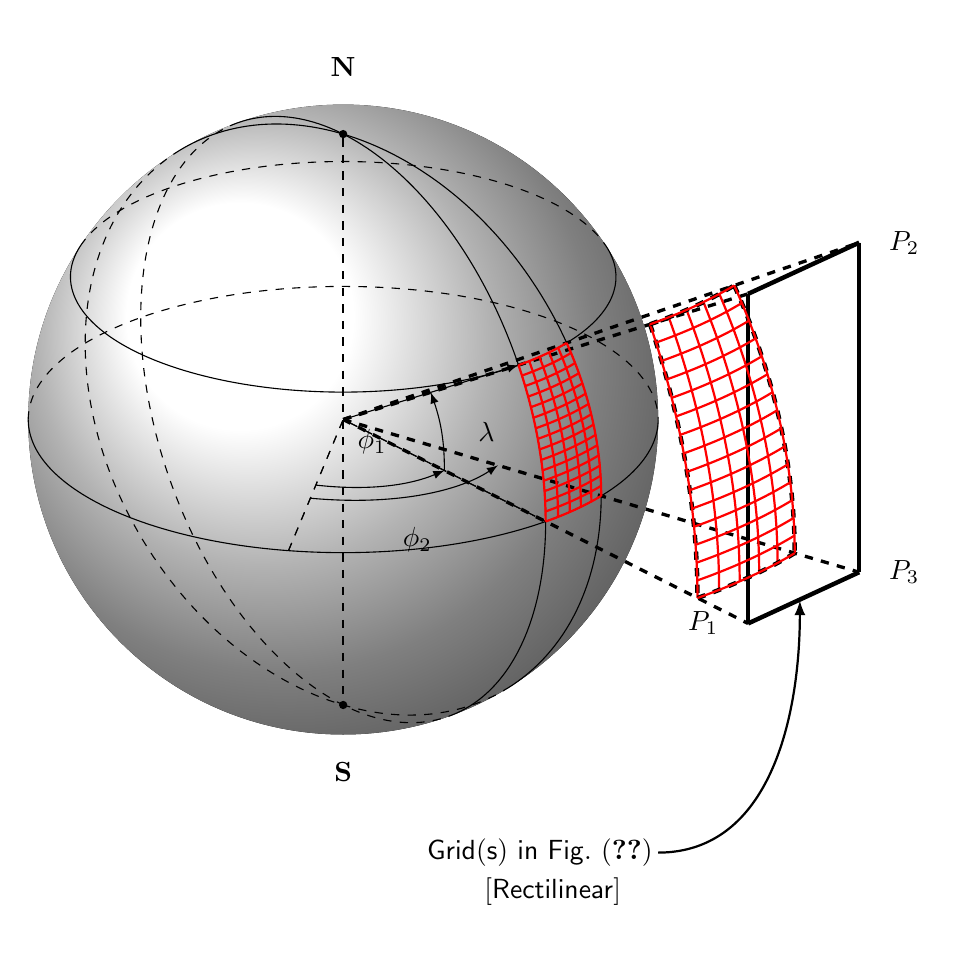
\begin{tikzpicture}[scale=1,every node/.style={minimum size=1cm}]
		%% some definitions
		
		\def\R{4} % sphere radius
		
		\def\angEl{25} % elevation angle
		\def\angAz{-100} % azimuth angle
		\def\angPhiOne{-50} % longitude of point P
		\def\angPhiTwo{-35} % longitude of point Q
		\def\angBeta{30} % latitude of point P and Q
		
		%% working planes
		
		\pgfmathsetmacro\H{\R*cos(\angEl)} % distance to north pole
		\LongitudePlaneE[xzplane]{\angEl}{\angAz}
		\LongitudePlaneE[pzplane]{\angEl}{\angPhiOne}
		\LongitudePlaneE[qzplane]{\angEl}{\angPhiTwo}
		\LatitudePlane[equator]{\angEl}{0}
		\fill[ball color=white!10] (0,0) circle (\R); % 3D lighting effect
		\coordinate (O) at (0,0);
		\coordinate[mark coordinate] (N) at (0,\H);
		\coordinate[mark coordinate] (S) at (0,-\H);
		\path[xzplane] (\R,0) coordinate (XE);
		
		%defining points outsided the area bounded by the sphere
		\path[qzplane] (\angBeta:\R+5.2376) coordinate (XEd);
		\path[pzplane] (\angBeta:\R) coordinate (P);%fino alla sfera
		\path[pzplane] (\angBeta:\R+5.2376) coordinate (Pd);%sfora di una quantità pari a 10 dopo la sfera
		\path[pzplane] (\angBeta:\R+5.2376) coordinate (Td);%sfora di una quantità pari a 10 dopo la sfera
		\path[pzplane] (\R,0) coordinate (PE);
		\path[pzplane] (\R+4,0) coordinate (PEd);
		\path[qzplane] (\angBeta:\R) coordinate (Q);
		\path[qzplane] (\angBeta:\R) coordinate (Qd);%sfora di una quantità pari a 10 dopo la sfera
		
		\path[qzplane] (\R,0) coordinate (QE);
		\path[qzplane] (\R+4,0) coordinate (QEd);%sfora di una quantità 10 dalla sfera sul piano equat.
		
		
		\DrawLongitudeCircle[\R]{\angPhiOne} % pzplane
		\DrawLongitudeCircle[\R]{\angPhiTwo} % qzplane
		\DrawLatitudeCircle[\R]{\angBeta}
		\DrawLatitudeCircle[\R]{0} % equator
		%labelling north and south
		\node[above=8pt] at (N) {$\mathbf{N}$};
		\node[below=8pt] at (S) {$\mathbf{S}$};
		
		\draw[-,dashed, thick] (N) -- (S);
		\draw[->] (O) -- (P);
		\draw[dashed] (XE) -- (O) -- (PE);
		\draw[dashed] (O) -- (QE);
		%connecting Points outside the sphere
		\draw[-,dashed,black,very thick] (O) -- (Pd);
		\draw[-,dashed,black,very thick] (O) -- (PEd);
		\draw[-,dashed,black,very thick] (O) -- (QEd);
		\draw[-,dashed,black,very thick] (O) -- (XEd);
		\draw[dashed] (XE) -- (O) -- (PE);
		%draw black thick flat grid
		\draw[-,ultra thick,black] (Pd) -- (PEd) node[below, left] {$P_1$};%verticale sinistro
		\draw[-,ultra thick,black] (PEd) -- (QEd)node[below, right] {$P_3$};%orizzontale inferiore
		\draw[-,ultra thick,black] (Pd)-- (XEd)node[above, right] {$P_2$};%orizzontale superiore    
		\draw[-,ultra thick,black] (XEd) -- (QEd);  
		
		\draw[pzplane,->,thin] (0:0.5*\R) to[bend right=15]
		node[midway,right] {$\lambda$} (\angBeta:0.5*\R);
		\path[pzplane] (0.5*\angBeta:\R) node[right] {$$};
		\path[qzplane] (0.5*\angBeta:\R) node[right] {$$};
		\draw[equator,->,thin] (\angAz:0.5*\R) to[bend right=30]
		node[pos=0.4,above] {$\phi_1$} (\angPhiOne:0.5*\R);
		\draw[equator,->,thin] (\angAz:0.6*\R) to[bend right=35]
		node[midway,below] {$\phi_2$} (\angPhiTwo:0.6*\R);
		\path[xzplane] (0:\R) node[below] {$$};
		\path[xzplane] (\angBeta:\R) node[below left] {$$};
		\foreach \t in {0,2,...,30} { \DrawLatitudeCirclered[\R]{\t} }
		\foreach \t in {130,133,...,145} { \DrawLongitudeCirclered[\R]{\t} }
		
		%drawing grids on the spere invoking DLongredd and DrawLongitudeCirclered
		
		\foreach \t in {130,145,...,145} { \DLongredd[\R+3]{\t} }
		\foreach \t in {130,133,...,145} { \DrawLongitudeCirclered[\R+3]{\t} }
		
		\foreach \t in {0,30,...,30} { \DLatred[\R+3]{\t} }
		\foreach \t in {0,2,...,30} { \DrawLatitudeCirclered[\R+3]{\t} }
		
		%labelling
		\draw[-latex,thick](4,-5.5)node[left]{$\mathsf{Grid(s)\ in\ Fig. \ (\ref{fig:Grid})}$}
		to[out=0,in=270] (5.8,-2.3);
		\draw[thick](3.6,-6)node[left]{$[\mathsf{Rectilinear}]$};
		
		\end{tikzpicture}
		\caption[Representation of spherical and regular computational grids used by SWAN]
		{Representation of spherical (red) and cartesian (black) co-ordinate systems. Latter 
			gives an example of unstructured grids. Both unstructured. Conversion from former 
			to latter involves a deformation factor which is acceptable within a given spatial limit. 
			For my case, only unstructured flat meshes are employed (\textit{Lisboa} Geodetic 
			datum: black grid on the right). Confront above represented points ($P_1,P_2,P_3$) with 
			Fig.(\ref{fig:Grid}). \\Mathematically frames change accordingly: see Eq.(\ref{eq:actbal2sph}).}
		\label{fig:frames}
	\end{figure}
	
	
	
\end{document}